\section{Use Case Scenarios}
\label{sec:usecasescenarios}

\begin{figure}[htb]
	\centering
	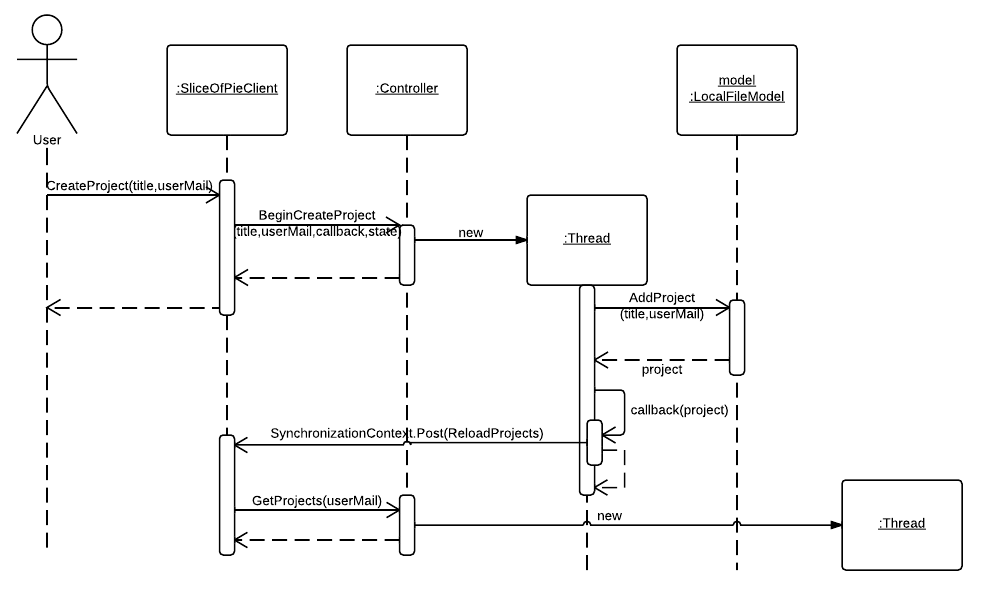
\includegraphics[width=1\textwidth]{Appendices/graphics/usecasescenario-createproject-local.png}
	\caption{Creating a project through a local client. This diagram details how the client requests a project
        creation, how the controller quickly returns to ensure that the UI does not lock up. Behind the scenes,
        the Controller has started a Thread (more specifically, it has commandeered one from the ThreadPool) that
        it is using to execute the requested command. The result is sent back to the Client through a callback,
        which changes the Synchronization Context (which thread executes the command) to the UI thread. The diagram
        stops before the next (automatically initiated) step continues: Reload of project state, to display an
        up-to-date list.}
	\label{fig:usecasescenario-01}
\end{figure}